\subsection{Metodolog�as para el desarrollo de software:}

Los softwares han sido parte de la vida cotidiana de la humanidad desde hace muchos a�os, pero su desarrollo comenz� de una manera muy desorganizada, ya que se basaba en actividades de codificar y arreglar los errores. Los softwares en su mayor�a eran creados sin seguir una l�nea de actividades, por lo que la estructura de estos pod�a variar frecuentemente. Pero como todo en la vida, llega un momento en que hay que organizar la forma en que se hacen las cosas, por lo que surgi� una alternativa llamada metodolog�a. Esta dictaba un proceso bien estructurado para la creaci�n de software, lo cual hac�a el desarrollo de estos m�s predictibles y eficientes.\\

Primero surgieron las metodolog�as tradicionales poseedoras de un plan de trabajo extenso, debido a la documentaci�n de los requerimientos del software, seguidos por la especificaci�n de la arquitectura y una representaci�n de alto nivel del software a desarrollar. Debido a la cantidad de trabajo a realizar, las metodolog�as tradicionales pasaron a ser conocidas como metodolog�as pesadas. Mayormente se utilizaban en software con un alto impacto, ya sea para la vida o la sociedad. Pero los proyectos que no pose�an un impacto tan notable, tambi�n deb�an utilizar las metodolog�as pesadas, por lo que el trabajo era muy lento y lleno de dificultades.\\

En respuesta al trabajo excesivo y minucioso en proyectos sin grandes repercusiones en la sociedad, nacieron las metodolog�as �giles, que fueron destinadas al desarrollo de software mediante la interacci�n con el cliente. Cambios en la estructura del proyecto de forma m�s seguida y un desarrollo r�pido, eran las caracter�sticas que m�s difer�an del prop�sito principal de las metodolog�as pesadas \citep{Awad2005}.\\


Dentro de las metodolog�as �giles se encuentran:

	\paragraph{ \ac{xp}:} Se caracteriza por los ciclos de desarrollo cortos, el incremento de los planes para el desarrollo del software, adem�s de la retroalimentaci�n que se establece con el cliente.
	\paragraph{ SCRUM:}
	 Describe la forma en que los miembros de equipo deben trabajar para poder obtener un sistema flexible en un entorno que var�a de manera constante.
 \paragraph{Agile Lite:}
		``(...)puede ser aplicada a cualquier proyecto, asumiendo que el trabajo a realizar se pueda dividir en peque�as acciones.'' \citep{AgileLiteHumanos}
		Utiliza ciclos de desarrollos cortos.\\


Con la ayuda de la informaci�n anteriormente expuesta, ya es hora de seleccionar una metodolog�a para el desarrollo del \cdis, pero antes, se deben poner en una balanza las caracter�sticas del mismo:


%	TABLE
\begin{table}[h]
	\centering
	\begin{tabular}{|l|l|l|}
		\hline
		\theader
		{ }                     & { �giles} & { Pesadas} \\ \hline
		Acercamiento            & X         &            \\ \hline
		\stripe
		Medici�n del objetivo   & X         &            \\ \hline
		Tama�o del proyecto     & X         &            \\ \hline
		\stripe
		Tipo de administraci�n  & X         &            \\ \hline
		Perspectiva de cambios  & X         &            \\ \hline
		\stripe
		Cultura del equipo      & X         &            \\ \hline
		Documentaci�n           & X         &            \\ \hline
		\stripe
		Orientada               & X         &            \\ \hline
		Ciclos de desarrollo    & X         &            \\ \hline
		\stripe
		Dominio de desarrollo   &           & X          \\ \hline
		Planificaci�n inicial   & X         &            \\ \hline
		\stripe
		Retorno de la inversi�n &           & X          \\ \hline
		Tama�o del equipo       & X         &            \\ \hline
		\stripe
		Total:                  & 11        & 2          \\ \hline
	\end{tabular}
	\caption{Resultado de la selecci�n de la metodolog�a}
	\label{tab:resultado}
\end{table}

Seg�n la tabla anterior, el software debe ser desarrollado siguiendo las pautas de las metodolog�as �giles, ya que cumple 11 de los 13 aspectos necesarios para decantarse por las mismas.

Dentro de las posibles metodolog�as �giles a seleccionar se encuentran \ac{xp}, Scrum y Agile Lite. Se decide utilizar \ac{xp}.

%	SUBSECTION
\subsubsection{Descripci�n de la metodolog�\ac{xp}}

``Es una Metodolog�a ligera de desarrollo de aplicaciones que se basa en la simplicidad, la comunicaci�n y la realimentaci�n del c�digo desarrollado''~\citep{VALLADAREZ2016}.

Objetivos de \ac{xp}:
\begin{itemize}
	\item La satisfacci�n del cliente.
	\item Potenciar el trabajo en equipo.
	\item Minimizar el riesgo actuando sobre las variables del proyecto: costo, tiempo, calidad, alcance.
\end{itemize}

Caracter�sticas:
\begin{itemize}
	\item Metodolog�a basada en prueba y error para obtener un software que funcione correctamente.
	\item Es orientada hacia quien produce y usa el software.
	\item Reduce el costo de cambio en todas las etapas del ciclo de vida de la aplicaci�n.
	\item Cliente bien definido.
	\item Los requisitos pueden cambiar.
\end{itemize}

\subsubsection{Artefactos de la metodolog�\ac{xp}}

\paragraph{Historias de usuario}

Las \ac{hu} representan una breve descripci�n del comportamiento del sistema. Se realizan por cada caracter�stica principal del sistema y son utilizadas para cumplir estimaciones de tiempo y el plan de lanzamientos, as� mismo reemplazan un gran documento de requisitos y presiden la creaci�n de las pruebas de aceptaci�n~\citep{VALLADAREZ2016}..

Cada \ac{hu} debe ser lo suficientemente comprensible y delimitada para que los programadores puedan implementarlas en unas semanas.



\paragraph{Tareas de ingenier�a}

Una \ac{hu} se descompone en varias tareas de ingenier�a, que describen las actividades que se realizar�n en cada \ac{hu}, as� mismo las tareas de ingenier�a se vinculan m�s al desarrollador, ya que permite tener un acercamiento con el c�digo~\citep{VALLADAREZ2016}.. 

%Esta puede ser vista en la tabla \ref{tab:ti}.
%
%\begin{table}[h]
%	\centering
%	\begin{tabular}{|l|l|}
%		\hline
%		\rowcolor[HTML]{C4BBD7} 
%		\multicolumn{2}{|c|}{\cellcolor[HTML]{C4BBD7}{Tarea de Ingenier�a}} \\ \hline
%		N�mero de tarea:  Identificador de la tarea. & \begin{tabular}[|c|]{@{}l@{}}  N�mero de historia: N�mero asignado \\ de la historia correspondiente. \end{tabular}\\ \hline
%		\stripe 
%		\multicolumn{2}{|l|}{\cellcolor[HTML]{EDEBF1}Nombre de Tarea: Describe de manera general dicha tarea.} \\ \hline
%		Tipo de tarea: Tipo al que corresponde dicha tarea. & \begin{tabular}[|c|]{@{}l@{}} Puntos estimados: N�meros de d�as necesarios \\ para desarrollar dicha tarea. \end{tabular} \\ \hline
%		\stripe 
%		Fecha Inicio: Fecha inicial de la creaci�n de dicha tarea. & Fecha Fin: Fecha de la culminaci�n de dicha tarea. \\ \hline
%		\multicolumn{2}{|l|}{Programador Responsable: Nombre del programador a cargo de desarrollar la tarea.} \\ \hline
%		\stripe 
%		\multicolumn{2}{|l|}{\cellcolor[HTML]{EDEBF1}Descripci�n: Informaci�n detallada de dicha tarea.} \\ \hline
%	\end{tabular}
%	\caption{Plantilla: Tarea de Ingenier�a.}
%	\label{tab:ti}
%\end{table}



\paragraph{Pruebas de aceptaci�n}

Antes de conocer en qu� consisten las pruebas de aceptaci�n, es necesario conocer los dos tipos de pruebas que  existen, hoy d�a, en la industria del software~\citep{Nidhra2012}:

\begin{itemize}
	\item \textbf{Caja negra}: Son las pruebas basadas en los requerimientos especificados y no es necesario examinar el c�digo.
	
	\item \textbf{Caja blanca}: Prueba aplicable �nicamente sobre el c�digo perteneciente a un software desarrollado. Son dise�ados desde el punto de vista del desarrollador. Es principalmente usado para detectar errores l�gicos en el c�digo de un programa. 
\end{itemize}

Las pruebas de aceptaci�n pertenecen a la categor�a de pruebas de caja negra y son de vital importancia para el �xito de una iteraci�n y el comienzo de la siguiente, con lo cual el cliente puede conocer el avance en el desarrollo del sistema y a los programadores lo que les resta por hacer. Adem�s, permite una retroalimentaci�n para el desarrollo de las pr�ximas historias de usuarios a ser entregadas. Estas son com�nmente llamadas pruebas del cliente, por lo que las realiza el encargado de verificar si las historias de usuarios de cada iteraci�n cumplen con la funcionalidad esperada~\citep{XPACT}. 
%
%Esta plantilla puede ser vista en la tabla \ref{tab:pa}.
%% Please add the following required packages to your document preamble:
%% \usepackage[table,xcdraw]{xcolor}
%% If you use beamer only pass "xcolor=table" option, i.e. \documentclass[xcolor=table]{beamer}
%\begin{table}[h]
%	\centering
%	\begin{tabular}{|l|l|}
%		\hline
%		\multicolumn{2}{|c|}{\cellcolor[HTML]{C4BBD7}Prueba de aceptaci�n} \\ \hline
%		\begin{tabular}[c]{@{}l@{}}C�digo: N� �nico, permite identificar \\ la prueba de aceptaci�n.\end{tabular} & \begin{tabular}[c]{@{}l@{}}N� Historia de Usuario: N�mero �nico \\ que identifica a la historia de usuario.\end{tabular} \\ \hline
%		\multicolumn{2}{|l|}{\cellcolor[HTML]{EDEBF1}\begin{tabular}[c]{@{}l@{}}Historia de Usuario: Nombre que indica de manera general \\ la descripci�n de la historia de usuario.\end{tabular}} \\ \hline
%		\multicolumn{2}{|l|}{\begin{tabular}[c]{@{}l@{}}Condiciones de Ejecuci�n: Condiciones previas que deben \\ cumplirse para realizar la prueba de aceptaci�n.\end{tabular}} \\ \hline
%		\multicolumn{2}{|l|}{\cellcolor[HTML]{EDEBF1}\begin{tabular}[c]{@{}l@{}}Entrada/Pasos de Ejecuci�n: Pasos que siguen los usuarios \\ para probar la funcionalidad de la historia de usuario.\end{tabular}} \\ \hline
%		\multicolumn{2}{|l|}{\begin{tabular}[c]{@{}l@{}}Resultado Esperado: Respuesta del sistema que el cliente espera, \\ despu�s de haber ejecutado una funcionalidad\end{tabular}} \\ \hline
%		\multicolumn{2}{|l|}{\cellcolor[HTML]{EDEBF1}\begin{tabular}[c]{@{}l@{}}Evaluaci�n de la Prueba: Nivel de satisfacci�n del cliente sobre \\ la respuesta del sistema. Los niveles son: Aprobada y No Aprobada.\end{tabular}} \\ \hline
%	\end{tabular}
%	\caption{Pruebas de aceptaci�n}
%	\label{tab:pa}
%\end{table}

\paragraph{Tarjetas \ac{crc}}

Las Tarjetas \ac{crc}, permiten conocer que clases componen el sistema y cuales interact�an entre s�.
%
%\begin{table}[h]
%	\centering
%	\begin{tabular}{|l|l|}
%		\multicolumn{2}{c}{\cellcolor[HTML]{C4BBD7}{Tarjeta CRC}} \\\hline
%		Nombre de la clase & \begin{tabular}[c]{@{}l@{}}N�mero de Historia: N�mero\\   de la historia de usuario correspondiente.\end{tabular} \\\hline
%		\multicolumn{2}{l}{\cellcolor[HTML]{EDEBF1}Responsabilidades: Atributos y operaciones de la clase.} \\ \hline
%	\end{tabular} 
%	\caption{Plantilla: Tarjeta CRC}
%	\label{tab:crc}
%\end{table}

\subsubsection{Fases de la metodolog�\ac{xp}}1

\begin{figure}[h]
	\centering
	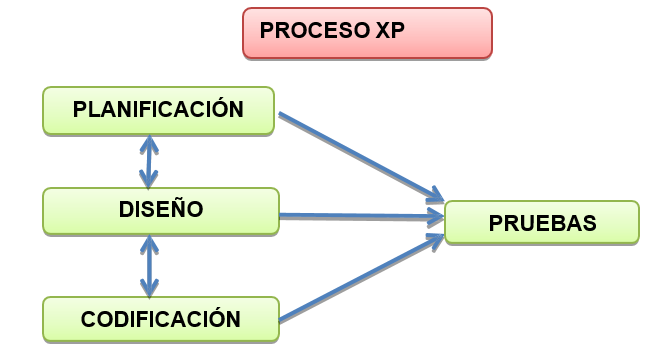
\includegraphics{xp.png}
	\caption{Fases de XP ~\citep{VALLADAREZ2016}.}
	\label{fig:xp}
\end{figure}

\begin{itemize}
	\item \textbf{Planificaci�n:} La Metodolog�\ac{xp} plantea la planificaci�n como un di�logo continuo entre las partes involucradas en el proyecto, incluyendo al cliente, a los programadores y a los coordinadores. El proyecto comienza recopilando las historias de usuarios, las que constituyen a los tradicionales casos de uso. Una vez obtenidas estas historias de usuarios, los programadores eval�an r�pidamente el tiempo de desarrollo de cada una, determinando as� el tiempo total de desarrollo del software.
	\item \textbf{Dise�o}: Especificaci�n de c�mo debe ser el Dise�o final de la aplicaci�n, haciendo �nfasis en que un Dise�o sencillo es m�s f�cil de implementar que uno complejo.
	\item \textbf{Codificaci�n}: Implementaci�n de los c�digos necesarios para satisfacer las historias de usuario.
	\item \textbf{Pruebas}: Una vez terminada la codificaci�n, se deben realizar las pruebas pertinentes a la misma.
\end{itemize}